\section{Robótica} \label{sect:robotica}
 
El presente trabajo se basa en la construcción de un robot humanoide, por lo tanto es importante definir qué es un robot, qué significa que sea humanoide y cuáles son algunos de sus componentes principales.

\begin{itemize}
\item{\textbf{Robótica:} Es el campo de la tecnología que se encarga de todas las tareas que se aplican a los robots.}

\item{\textbf{Robot:} Es un agente f\'isico que realiza tareas manipulando su ambiente.
Generalmente un robot está equipado con actuadores y sensores. Una posible divisi\'on para categorizarlos es por su forma, en primera instancia están los manipuladores o brazos rob\'oticos que normalmente están anclados a su espacio de trabajo y generalmente desempeñan tareas en f\'abricas o l\'ineas de emsamblaje; como su nombre lo describe, tienen forma de brazo. La siguiente categor\'ia se refiere a robots móviles, su principal caracter\'itica es que tienen la capacidad de desplazamiento por lo cual poseen piernas, ruedas o cualquier mecanismo que le permita desplazarse, generalmente en esta clasificaci\'on se incluyen robots que pueden realizar una gran diversidad de tipos de tareas. La \'ultima divisi\'on es la categor\'ia mixta, son aquellos robots que poseen caracter\'isticas tanto de brazos rob\'oticos como de móviles, en ella se incluye a los robots humanoides que, como su nombre lo indica están hechos a semejanza del hombre. Sus tareas suelen requerir un poco más de esfuerzo ya que en la manipulaci\'on de objetos no poseen la ventaja del anclaje que tienen los brazos rob\'oticos. Los robots reales suelen enfrentarse a ambientes parcialmente observables, estoc\'asticos, din\'amicos y continuos \cite{peterNorvig}.}

%Son agentes físicos que ejecutan tareas para manipular el mundo físico. Para ello deden estar equipados con actuadores y sensores \cite{peterAndNorvig}. La apariencia no es una característica útil para la definición de un robot \cite{AiRobotics}, por lo tanto puede ser de diferentes formas, ya sea con ruedas, con piernas o ninguna de ellas. Una de las formas que puede adoptar un robot es la de humano, de hecho en la cultura popular el término ``robot" generalmente connota una apariencia humana \cite{AiRobotics}. Según el diccionario de la Universidad de Oxford,  el término humanoide se refiere a tener una apariencia o característica parecida a la de un ser humano \cite{oxfordRobotics}, por lo tanto a los robots con forma de humano se les denomina robots humaniodes.}    

\item{\textbf{Sensores:} Son dispositivos incorporados a los robots que obtienen información del ambiente. Algunos miden las magnitudes de los cambios externos que ocurren, como las c\'amaras, los sonares, entre otros. Tambi\'en existen los que miden cambios internos, como los giroscopios y aceler\'ometros. En general un sensor es una interfaz de percepci\'on entre el ambiente y el robot \cite{peterNorvig}.}

%Son los dispositivos encargados de percibir el ambiente que rodea al robot. Según Murphy R.R estos miden algún atributo del mundo. Un sensor recibe energía del entorno (sonido, luz, presión, temperatura) y transmite una señal a una pantalla o computador ya sea de forma análoga o digital \cite{AiRobotics}. Algunos sensores son: cámaras, giroscopios, sensores de proximidad, entre otros.}

\item{\textbf{Actuadores:} Son dispositivos que realizan cambios f\'isicos en el medio ambiente. Por ejemplo ruedas, piernas, pinzas, entre otros \cite{peterNorvig}.}

\item{\textbf{Servomotor:}  Es un motor eléctrico, un actuador, que permite controlar su velocidad y posici\'on  \cite{AiRobotics}. }

 %http://www.ceiarteuntref.edu.ar/badarte/node/112

\item{\textbf{Giroscopio:} Es un sensor propioceptivo que informa al robot de su estado de velocidad de giro en uno o varios ejes, pertence a los sensores de inercia \cite{peterNorvig}. Mide el momento angular y se utiliza para mantener orientaci\'on o equilibrio.}

%Es un sensor utilizado para medir y mantener la orientación, se mide a través del momento angular \cite{gyro1}. }
\end{itemize}

%****************************************************************************************/
\section{Robótica Inteligente} \label{sect:AgentesInteligentes}

Es importante diferenciar cuando un robot es inteligente o no. Cuando un robot es operado a distancia, y no es capaz de cumplir su tarea sin la intervención de un humano, entonces no se considera  inteligente. Tampoco se considera inteligente si las tareas que ejecuta se hacen sin sentido o de manera repetitiva. En cambio cuando un robot puede interactuar con el mundo de manera autónoma se considera que es un robot o agente inteligente \cite{AiRobotics}. Existen diferentes estrategias o enfoques de cómo aplicar la inteligencia en un robot. Esta sección se dedica a describir los enfoques que se han definido como paradigmas. 

Existen tres paradigmas. Estos serán descritos en base a los conceptos básicos de la robótica: percibir, planificar y actuar. Percibir se refiere al procesamiento de la información obtenida de los sensores del robot. Planificar es, cuando con la percepción, se crea un conocimiento del mundo y se organizan la tareas que el robot debe realizar para lograr un objetivo. Por último, actuar consiste en realizar tareas con los actuadores del robot para modificar el entorno \cite{AiRobotics}. 

\subsection{Paradigma Jerárquico}

Este paradigma es secuencial y ordenado. Primero el robot percibe el mundo y construye un mapa general. En base al mapa ya percibido y sin percibir m\'as por el momento, el robot planifica todas tareas necesarias para lograr la meta. Luego ejecuta la secuencia de actividades según su planificaci\'on. Una vez culminada la secuencia se repite el ciclo percibiendo el mundo, planificando y actuando \cite{AiRobotics}. Una representación visual del orden que sigue este paradigma se muestra en la imagen \ref{fig:jerarquico}.

\begin{figure}[hbtp]
\centering
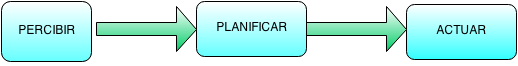
\includegraphics[scale=0.7]{imagenes/jerarquico.png} 
\caption{Paradigma Jer\'arquico}
\label{fig:jerarquico}
\end{figure}


\subsection{Paradigma Reactivo}
El paradigma reactivo omite por completo el componente de la planificación y s\'olo se basa en percibir y actuar. El robot puede mantener un conjunto de pares percibir-actuar como se muestra en la figura \ref{fig:reactivo}, \'estos son llamados comportamientos y se ejecutan como procesos concurrentes. Un comportamiento toma datos de la percepción del mundo y los procesa para tomar la mejor acción independientemente de los otros procesos \cite{AiRobotics}.

\begin{figure}[hbtp]

\centering
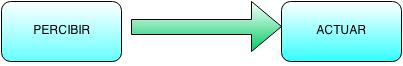
\includegraphics[scale=0.7]{imagenes/reactivo.jpg} 
\caption{Paradigma Reactivo}
\label{fig:reactivo}
\end{figure}


\subsection{Paradigma Híbrido}
El paradigma híbrido es una mezcla de los dos paradigmas anteriores. Primero se planifica cúal es la mejor manera de cumplir el objetivo principal, descomponiendo la tarea general en sub-tareas y decidiendo qué comportamientos sirven para cumplir cada una. De allí en adelante se ejecutan los comportamientos (percibiendo y actuando), hasta que el plan sea ejecutado, si es necesario se puede volver a planificar. Vale la pena acotar que la información de los sensores se encuentra siempre disponible para el planificador, de manera que pueda crear un modelo del mundo y tomar decisiones en base a él  \cite{AiRobotics}. Esto se ilustra en la figura \ref{fig:hibrido}
\begin{figure}[hbtp]

\centering
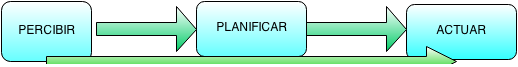
\includegraphics[scale=0.7]{imagenes/hibrido.png} 
\caption{Paradigma H\'ibrido}
\label{fig:hibrido}
\end{figure}
